\textbf{Исходный текст:} \\
    A magic square of order n is an arrangement of n\^~2 numbers,
    usually distinct integers, in a square, such that the n numbers
    in all rows, all columns, and both diagonals sum to the same constant.
    A magic square contains the integers from 1 to n\^~2. \\
    The constant sum in every row, column and diagonal is called the magic
    constant or magic sum, M. The magic constant of a normal magic square
    depends only on n and has the following value: M = n (n\^~2 + 1) / 2.

\textbf{Зашифрованный текст:} \\
    cgs orar aa2loamn ,we eb he,ru\^~o m asio ch ltgsrqnfsrets rettdl eras(
    dohTnl hninahte   enn  oayTig  cnbncnhepa.cnr
    ~aoauimai t e M oe.emt n u g= sdf cgv2h  ,isnsaMa o,iae\^~tAms  tim he
    mgi n  uns,c  : rtuadn s.smren2 edansm iont ueri\^~nAunua  d tinslbatn
    r.laqtcenm aalomus fe2a ssihau1ttacuqidodvn ngt s nsn ns   r  coa n
    monol nayto/ icmdmtocogla  ln  gn  eunr cai enlef)nogrllafe ed,hiamo1i
    aclot ram st ue  wymiocssruahw ,sge+ol g anoeqstotsunr lnlatc 

Результаты работы программы представлены на рисунках~\ref{ris:encode-test-4}-\ref{ris:decode-test-4}.

\vspace{\baselineskip}
\begin{figure}[H]
\center{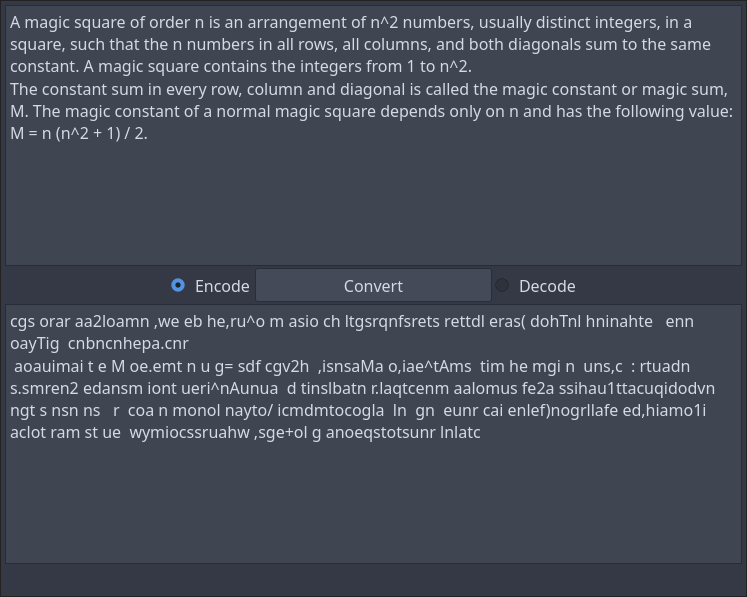
\includegraphics[width=0.7\linewidth]{figures/encode-test-4}}
    \caption{Шифрование}
\label{ris:encode-test-4}
\end{figure}

\vspace{\baselineskip}
\begin{figure}[H]
\center{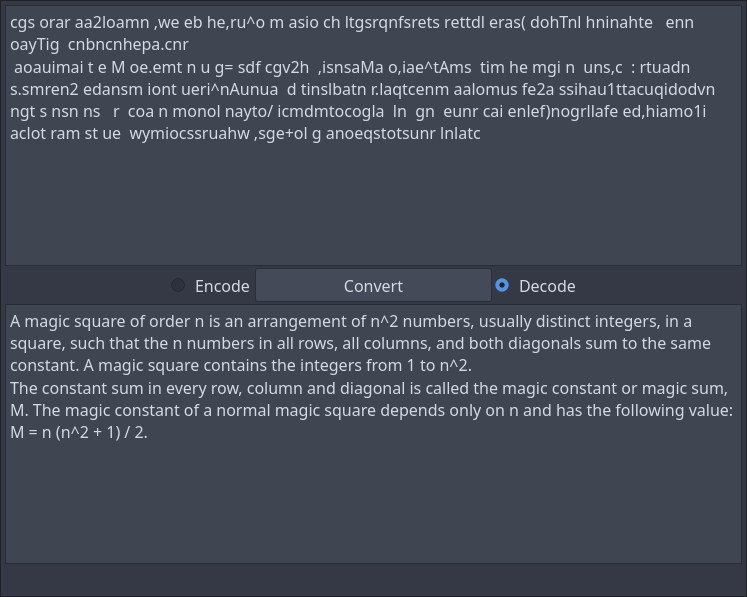
\includegraphics[width=0.7\linewidth]{figures/decode-test-4}}
    \caption{Расшифрование}
\label{ris:decode-test-4}
\end{figure}
